% Options for packages loaded elsewhere
\PassOptionsToPackage{unicode}{hyperref}
\PassOptionsToPackage{hyphens}{url}
%
\documentclass[
  english,
  man,11pt,floatsintext]{apa7}
\usepackage{lmodern}
\usepackage{amssymb,amsmath}
\usepackage{ifxetex,ifluatex}
\ifnum 0\ifxetex 1\fi\ifluatex 1\fi=0 % if pdftex
  \usepackage[T1]{fontenc}
  \usepackage[utf8]{inputenc}
  \usepackage{textcomp} % provide euro and other symbols
\else % if luatex or xetex
  \usepackage{unicode-math}
  \defaultfontfeatures{Scale=MatchLowercase}
  \defaultfontfeatures[\rmfamily]{Ligatures=TeX,Scale=1}
\fi
% Use upquote if available, for straight quotes in verbatim environments
\IfFileExists{upquote.sty}{\usepackage{upquote}}{}
\IfFileExists{microtype.sty}{% use microtype if available
  \usepackage[]{microtype}
  \UseMicrotypeSet[protrusion]{basicmath} % disable protrusion for tt fonts
}{}
\makeatletter
\@ifundefined{KOMAClassName}{% if non-KOMA class
  \IfFileExists{parskip.sty}{%
    \usepackage{parskip}
  }{% else
    \setlength{\parindent}{0pt}
    \setlength{\parskip}{6pt plus 2pt minus 1pt}}
}{% if KOMA class
  \KOMAoptions{parskip=half}}
\makeatother
\usepackage{xcolor}
\IfFileExists{xurl.sty}{\usepackage{xurl}}{} % add URL line breaks if available
\IfFileExists{bookmark.sty}{\usepackage{bookmark}}{\usepackage{hyperref}}
\hypersetup{
  pdfauthor={Alexander Enge1},
  pdflang={en-EN},
  pdfkeywords={keywords},
  hidelinks,
  pdfcreator={LaTeX via pandoc}}
\urlstyle{same} % disable monospaced font for URLs
\usepackage{graphicx,grffile}
\makeatletter
\def\maxwidth{\ifdim\Gin@nat@width>\linewidth\linewidth\else\Gin@nat@width\fi}
\def\maxheight{\ifdim\Gin@nat@height>\textheight\textheight\else\Gin@nat@height\fi}
\makeatother
% Scale images if necessary, so that they will not overflow the page
% margins by default, and it is still possible to overwrite the defaults
% using explicit options in \includegraphics[width, height, ...]{}
\setkeys{Gin}{width=\maxwidth,height=\maxheight,keepaspectratio}
% Set default figure placement to htbp
\makeatletter
\def\fps@figure{htbp}
\makeatother
\setlength{\emergencystretch}{3em} % prevent overfull lines
\providecommand{\tightlist}{%
  \setlength{\itemsep}{0pt}\setlength{\parskip}{0pt}}
\setcounter{secnumdepth}{-\maxdimen} % remove section numbering
% Make \paragraph and \subparagraph free-standing
\ifx\paragraph\undefined\else
  \let\oldparagraph\paragraph
  \renewcommand{\paragraph}[1]{\oldparagraph{#1}\mbox{}}
\fi
\ifx\subparagraph\undefined\else
  \let\oldsubparagraph\subparagraph
  \renewcommand{\subparagraph}[1]{\oldsubparagraph{#1}\mbox{}}
\fi
% Manuscript styling
\usepackage{upgreek}
\captionsetup{font=singlespacing,justification=justified}

% Table formatting
\usepackage{longtable}
\usepackage{lscape}
% \usepackage[counterclockwise]{rotating}   % Landscape page setup for large tables
\usepackage{multirow}		% Table styling
\usepackage{tabularx}		% Control Column width
\usepackage[flushleft]{threeparttable}	% Allows for three part tables with a specified notes section
\usepackage{threeparttablex}            % Lets threeparttable work with longtable

% Create new environments so endfloat can handle them
% \newenvironment{ltable}
%   {\begin{landscape}\begin{center}\begin{threeparttable}}
%   {\end{threeparttable}\end{center}\end{landscape}}
\newenvironment{lltable}{\begin{landscape}\begin{center}\begin{ThreePartTable}}{\end{ThreePartTable}\end{center}\end{landscape}}

% Enables adjusting longtable caption width to table width
% Solution found at http://golatex.de/longtable-mit-caption-so-breit-wie-die-tabelle-t15767.html
\makeatletter
\newcommand\LastLTentrywidth{1em}
\newlength\longtablewidth
\setlength{\longtablewidth}{1in}
\newcommand{\getlongtablewidth}{\begingroup \ifcsname LT@\roman{LT@tables}\endcsname \global\longtablewidth=0pt \renewcommand{\LT@entry}[2]{\global\advance\longtablewidth by ##2\relax\gdef\LastLTentrywidth{##2}}\@nameuse{LT@\roman{LT@tables}} \fi \endgroup}

% \setlength{\parindent}{0.5in}
% \setlength{\parskip}{0pt plus 0pt minus 0pt}

% Overwrite redefinition of paragraph and subparagraph by the default LaTeX template
% See https://github.com/crsh/papaja/issues/292
\makeatletter
\renewcommand{\paragraph}{\@startsection{paragraph}{4}{\parindent}%
  {0\baselineskip \@plus 0.2ex \@minus 0.2ex}%
  {-1em}%
  {\normalfont\normalsize\bfseries\itshape\typesectitle}}

\renewcommand{\subparagraph}[1]{\@startsection{subparagraph}{5}{1em}%
  {0\baselineskip \@plus 0.2ex \@minus 0.2ex}%
  {-\z@\relax}%
  {\normalfont\normalsize\itshape\hspace{\parindent}{#1}\textit{\addperi}}{\relax}}
\makeatother

% \usepackage{etoolbox}
\makeatletter
\patchcmd{\HyOrg@maketitle}
  {\section{\normalfont\normalsize\abstractname}}
  {\section*{\normalfont\normalsize\abstractname}}
  {}{\typeout{Failed to patch abstract.}}
\patchcmd{\HyOrg@maketitle}
  {\section{\protect\normalfont{\@title}}}
  {\section*{\protect\normalfont{\@title}}}
  {}{\typeout{Failed to patch title.}}
\makeatother
\shorttitle{Semantic Knowledge and Unfamiliar Objects}
\keywords{keywords\newline\indent Word count: X}
\usepackage{csquotes}
\usepackage{setspace}
\AtBeginEnvironment{tabular}{\doublespacing}
\AtBeginEnvironment{lltable}{\doublespacing}
\AtBeginEnvironment{tablenotes}{\doublespacing}
\captionsetup[table]{font={stretch=1.5}}
\captionsetup[figure]{font={stretch=1,scriptsize}}
\raggedbottom
\ifxetex
  % Load polyglossia as late as possible: uses bidi with RTL langages (e.g. Hebrew, Arabic)
  \usepackage{polyglossia}
  \setmainlanguage[]{english}
\else
  \usepackage[shorthands=off,main=english]{babel}
\fi

\title{Event-Related Potentials of the Semantically\\
Informed Perception of Unfamiliar Objects}
\author{Alexander Enge\textsuperscript{1}}
\date{}


\authornote{

Alexander Enge, Department of Psychology, Humboldt-Universität zu Berlin, Germany, \url{https://orcid.org/0000-0003-0100-2297}, student no. 581331.

The thesis was handed in December 18, 2020 and has been supervised by Prof.~Dr.~Rasha Abdel Rahman, Humboldt-Universität zu Berlin, Germany, and Prof.~Dr.~Franziska Süß, Fachhochschule des Mittelstands, Bamberg, Germany.

Correspondence concerning this article should be addressed to Alexander Enge, Rudower Chaussee 18, 12489 Berlin. E-mail: \href{mailto:alexander.enge@hu-berlin.de}{\nolinkurl{alexander.enge@hu-berlin.de}}

}

\affiliation{\vspace{0.5cm}\textsuperscript{1} Humboldt-Universität zu Berlin}

\abstract{
Abstract goes here.
}



\begin{document}
\maketitle

How does our perception of an object change as soon as we discover what it is for? In this study, we presented participants with unfamiliar objects, preceded in half of the cases by valid information about their function, leading to semantically informed perception, and in the other half of the cases by misleading information, leading to naive perception. Capitalizing on the high temporal resolution of event-related brain potentials (ERPs), we investigated at which stages in the processing hierarchy semantically informed and naive perception of visual objects differed from one another.

The claim that higher-level cognitive capacities such as knowledge or language can modulate lower-level perceptual processes has been the source of a long-standing debate. This debate revolves around the question whether or not our perception of the (visual) world should be thought of as an encapsulated module being completely determined by the visual input reaching our retina. According to the former view, higher-level mental states and functions are not able to penetrate perception and kick in only after lower-level perceptual analysis of the visual input has taken pace (Firestone \& Scholl, 2016; Fodor, 1984, 1983; Machery, 2015; Pylyshyn, 1999). Conversely, this view is challenged by theoretical and empirical work suggesting that perceptual processing dynamically interacts with other aspects of cognition from early on (Churchland, 1988; Churchland et al., 1994; Collins \& Olson, 2014; Lupyan, 2012, 2015; Lupyan et al., 2020; Thierry, 2016; Vetter \& Newen, 2014). These aspects may include transient states such as emotions (e.g.~Phelps et al., 2016; Bocanegra \& Zeelenberg, 2009) or intentions (Balcetis \& Dunning, 2010; Cole et al., 2012) as well as learned capacities such as language (e.g.~Boutonnet \& Lupyan, 2015; Maier \& Abdel Rahman, 2018; Mo et al., 2011) or declarative knowledge about faces (e.g.~Abdel Rahman, 2011; Eiserbeck \& Abdel Rahman, 2020; Suess et al., 2015) and objects (e.g.~Abdel Rahman \& Sommer, 2008; Lin \& Murphy, 1997; Weller et al., 2019). Despite this wealth of empirical evidence, critics of the idea that cognitive functions can penetrate perception have remained sceptical, pointing out important methodological shortcomings in large parts of this literature (Firestone \& Scholl, 2016).

One productive way of investigating top-down effects of cognition on perception while addressing some of these concerns is through neurophysiological recording methods such as ERPs: Their high temporal resolution allows for a direct test of which processing stages---perceptual and/or postperceptual---are influenced by higher-level capacities such as semantic knowledge. This is because when participants are presented with visual stimuli, their averaged brain responses show characteristic deflections (ERP components), each of them with its typical polarity (positive or negative), peak latency, spatial scalp distribution, and functional role(s).

The visual P1 component refers to a positive deflection peaking approximately 100--150 ms after stimulus onset at occipital channels. It is generated by multiple sources in the extrastriatal cortices of the middle occipital and fusiform gyri (Di Russo et al., 2001; Foxe \& Simpson, 2002; Mangun, 1995). The P1 is mostly thought to reflect the processing of low-level visual characteristics of the stimulus (such as size, luminance, and contrast; Di Russo et al., 2001; Johannes et al., 1995; Luck, 2014), which is why it being modulated by higher-level cognitive capacities would challenge a purely bottom-up, encapsulated conception of visual perception. It should be noted, however, that the P1 is reliably modulated by spatial (Luck et al., 2000; Mangun, 1995; Mangun \& Hillyard, 1991) and non-spatial (Taylor, 2002) attention.

The visual N170 (or N1) component refers to the negative deflection following the P1 and is maximal around 150--200 ms after stimulus onset at occipito-temporal channels. While still influenced by visual parameters of the stimulus (Johannes et al., 1995), it is also sensitive to selective attention, at least when participants are required to discriminate between different visual stimuli (Mangun \& Hillyard, 1991; Vogel \& Luck, 2000). Importantly, the N170 is enlarged (i.e.~more negative) in response to faces (Bentin et al., 1996; Rossion \& Jacques, 2011) and other visual stimuli for which one happens to be an expert (e.g.~birds, dogs, or cars; I. Gauthier, Curran, et al., 2003; Tanaka \& Curran, 2001). This category selectivity seems to reflect both the processing of individual visual features of the respective objects (including faces) as well as their configuration (Eimer et al., 2011; Jacques \& Rossion, 2010; Rossion et al., 1999; Sagiv \& Bentin, 2001). Thus, a modulation of the N170 by cognitive capacities such as knowledge would suggest these factors having an influence on higher-level, holistic perception of the visual stimuli.

Finally, the N400 component refers to more negative ERP amplitudes when stimuli require more as compared to less resources for semantic processing or integration (Kutas \& Federmeier, 2011; Lau et al., 2008; Rabovsky et al., 2018), starting approximately 300 ms after stimulus onset and being most pronounced at centro-parietal channels. A modulation of this component by cognitive capapacities such as knowedge can be taken as evidence for a post-perceptual influence on stimulus processing.

Previous studies have focused on these and other ERP components to investiage which processing stages are indeed influenced by knowledge or expertise in the domain of visual objects (Abdel Rahman \& Sommer, 2008; Gratton et al., 2009; Maier et al., 2014; Maier \& Rahman, 2019; Rossion et al., 2002, 2004; Samaha et al., 2018; Tanaka \& Curran, 2001; Weller et al., 2019). Together, they suggest that not only higher-level semantic ERPs like the N400 component are influenced by acquiring semantic information about objects, but also early components that typcially reflect bottom-up visual processing. This was the case, for instance, when participants were presented with a range of unfamiliar objects, receiving in-depth verbal descriptions about their function for half of the objects and irrelevant verbal information (cooking recipes) for the other half of the objects (Abdel Rahman \& Sommer, 2008, Experiment 1). After this learning phase, the same objects were presented in three different ERP tasks which did not require explicit access to any of the learned semantic information. In all three tasks, ERP amplitudes in response to objects for which in-depth knowledge had been acquired differed from those in response to objects for which this has not been the case. Crucially, these differences occurred not just in the N400 component, indexing a modulation of post-perceptual semantic processing, but also in the P1 component, suggesting a top-down modulation of lower-level perceptual processing. Of note, the ERPs in the in-depth knowledge condition were qualitatively similar to those for untrained but well-known objects. The modulation of the P1 component was also replicated when the same objects were presented under circumstances of limited attentional resources in an attentional blink paradigm (Weller et al., 2019). Of note, the (neurophysiological) differences in P1 amplitudes between objects with in-depth versus minimal knowledge were correlated with (behavioral) differences in their detection rate during the attentional blink, which can be taken as further evidence of an influence of semantic knowledge on the early visual perception of unfamiliar objects.

A complementary approach has been taken in a recent study investigating the ERPs in response to familiar (rather than unfamiliar) objects, which were rendered difficult to recognize by converting them to two-tone, \enquote{Mooney} images (Samaha et al., 2018, Experiment 4). Here, participants were trained with meaningful verbal cues, telling them what kind of objects they should look for in the image beforehand, or with a non-meaningful perceptual task, familiarizing them with the images but not with their semantic content. When the EEG was measured in a separate delayed matching task later on, the two types of training led to differential effects, again suggesting a modulation of lower-level visual perception: Over left posterior electrodes, P1 amplitudes were larger and alpha power was higher for meaning-trained images of objects than for perceptually-trained images of objects. This alternative approach further coroborates an early influence of semantic information on visual object perception.

All the previously mentioned studies have in common that they investigated the effects of semantic knoweldge on object perception only \emph{after} an extensive learning phase (Abdel Rahman \& Sommer, 2008; I. Gauthier, James, et al., 2003; Maier et al., 2014; Maier \& Rahman, 2019; Rossion et al., 2002, 2004; Samaha et al., 2018; Weller et al., 2019). Participants performed one or multiple training session where they encountered each object together with its respective label or description multiple times. The EEG was usually not measured---or at least not analyzed and reported---during these training sessions, which sometimes took place on a separate day (Abdel Rahman \& Sommer, 2008; Maier et al., 2014; Maier \& Rahman, 2019) or were spread out across multiple days or weeks (Rossion et al., 2002, 2004). While designs with such substantive training maximize the chances of detecting even subtle top-down effects of the knowledge acquired, they necessarily leave at least three important conceptual questions unresolved.

The first question is if we can detect any electrophysiological correlates of semantic insight, i.e.~the critical presentation during which an understanding of the previously unfamiliar object is happening, instead of asking if this understanding leads to differential effects in an orthogonal task later on. The second question is how much learning is actually necessary before reliable top-down effects of knowledge (such as~on object-related P1 amplitudes) can be obtained: Does it actually take dozens of repitions per object or may a single exposure to the object together with the relevant semantic information be enough? The third and closely related question is about the nature of knowledge effects on perception: Are they reflecting genuine top-down effects of semantics, altering perception online (while the object is being perceived), or do they merely reflect the (re-)activation of stored representations of the objects, having been altered throughout the learning process (Haber, 1966)? By measuring the ERPs before, during, and after participants received semantic hints about unfamiliar objects, we hope to provide tentative answers to all three of these questions.

In the two experiments subsequently reported, participants were presented with real-word objects that were presumed to be unfamiliar to most of them. They first viewed each of these objects once without any semantic information. This part served as a naive baseline to outrule that ERPs would differ in response to the objects based solely on their low-level visual differences. Next, participants viewed each unfamiliar object for a second time, now preceded by verbal keywords. These keywords could either correctly describe the object's typical function, thus making it possible for participants to understand what kind of object they are viewing, or mislead them by describing the function of a different object, thus keeping the perception of the object semantically naive. During this \enquote{insight} part, we were able measure the online influence of semantic knowledge on object-evoked ERPs as it happened. Finally, the objects were presented for a third time (without keywords, as in the first part) to investigate downstream effects of having acquired semantic knowledge about them, thus mimicking previous studies (e.g.~Abdel Rahman \& Sommer, 2008, p. @samaha2018; Weller et al., 2019). In all three parts, we compared the influences of semantic information on ERPs associated with lower-level visual perception (P1 component, 100--150 ms), higher-level visual perception (N170 component, 150--200 ms), and semantic processing (400--700 ms).

\hypertarget{experiment-1}{%
\section{Experiment 1}\label{experiment-1}}

\hypertarget{methods}{%
\subsection{Methods}\label{methods}}

\hypertarget{participants}{%
\subsubsection{Participants}\label{participants}}

Participants for Experiment 1 were 24 German native speakers (13 female, 11 male) with a mean age of 24 years (range 18 to 31) and no history of psychological disorder or treatment. No a priori power analysis was carreid out and the sample size was chosen according to the default for EEG studies in our lab at the time of data collection. All participants were right-handed according to the Edinburgh inventory (Oldfield, 1971) and reported normal or corrected-to-normal vision. They gave written informed consent before starting the experiment and received a compensation of €8 per hour for participating. All experiments subsequently reported were carried out in accordance with the Declaration of Helsinki and approved by the local ethics committee.

\hypertarget{materials-and-procedure}{%
\subsubsection{Materials and Procedure}\label{materials-and-procedure}}

Stimuli for Experiments 1 and 2 consisted of 240 grayscale photographs of real-world objects, 120 of which were well-known everyday objects (e.g.~a bicycle, a toothbrush), serving as filler stimuli of no interest, whereas the other 120 were rare objects presumed to be unfamiliar for the majority of participants (e.g.~a galvanometer, an udu drum). A list of these unfamiliar objects can be found in Appendix A. All stimuli were presented on a light blue background with a size of 207 × 207 pixels on a 19-inch LCD monitor with a resolution of 1,280 × 1,024 pixels and a refresh rate of 75 Hz. At a standardized viewing distance of 90 cm, the images of the objects subtended approximately 3.9 degrees of participants' horizontal and vertical visual angle.

For each unfamiliar object, a pair of keywords---a noun and a verb---was selected describing the object's typical function or use in a way that could typically be related to its visual features and their configuration (e.g.~current--measuring, pottery--drumming). As our central experimental manipulation, the presentation of each unfamiliar object was preceded by its correctly matching keywords for half of the objects, whereas the other half were preceded by non-matching keywords belonging to one of the other objects. The matching keywords were expected to induce semantically informed perception (i.e.~participants suddenly understanding what kind of object they were viewing), whereas the non-matching keywords were expected hamper such an effect and keep the perception of the object semantically naive. All participants saw each unfamiliar object in only one of the two conditions and the assignment of objects to conditions was counterbalanced across participants. The experiment was programmed and displayed using Presentation® software (Neurobehavioral Systems, Inc., Berkeley, CA, www.neurobs.com).

Each experimental session consisted of three parts (Figure \ref{fig:exp1-plot}A). In the \emph{pre-insight} part (Part I), after written informed consent had been obtained and the EEG had been prepared, all 240 familiar and unfamiliar objects were presented once in random order and without any keywords. Each trial consisted of a fixation cross presented in the middle of the screen for 0.5 s, followed by the presentation of the object until participants made a response or until a time out after 3 s. The inter-trial interval until the presentation of the next fixation cross was 0.5 s and participants took a self-timed break after each block of 60 objects. The task, which was kept the same throughout all parts and experiments, was to classify each object using one of four response alternatives: (a) \enquote{I know what this is or have a strong assumption,} (b) \enquote{I have an assumption what this is,} (c) \enquote{I have rather no assumption what this is,} or (d) \enquote{I do not know what this is and have no assumption.} Participants were asked to respond as quickly and as accurately as possible by pressing one out of four buttons with the index or middle finger of their left or right hand, respectively. The mapping of the rating scale to the four buttons (left to right or right to left) was counterbalanced across participants.



\begin{figure}

{\centering 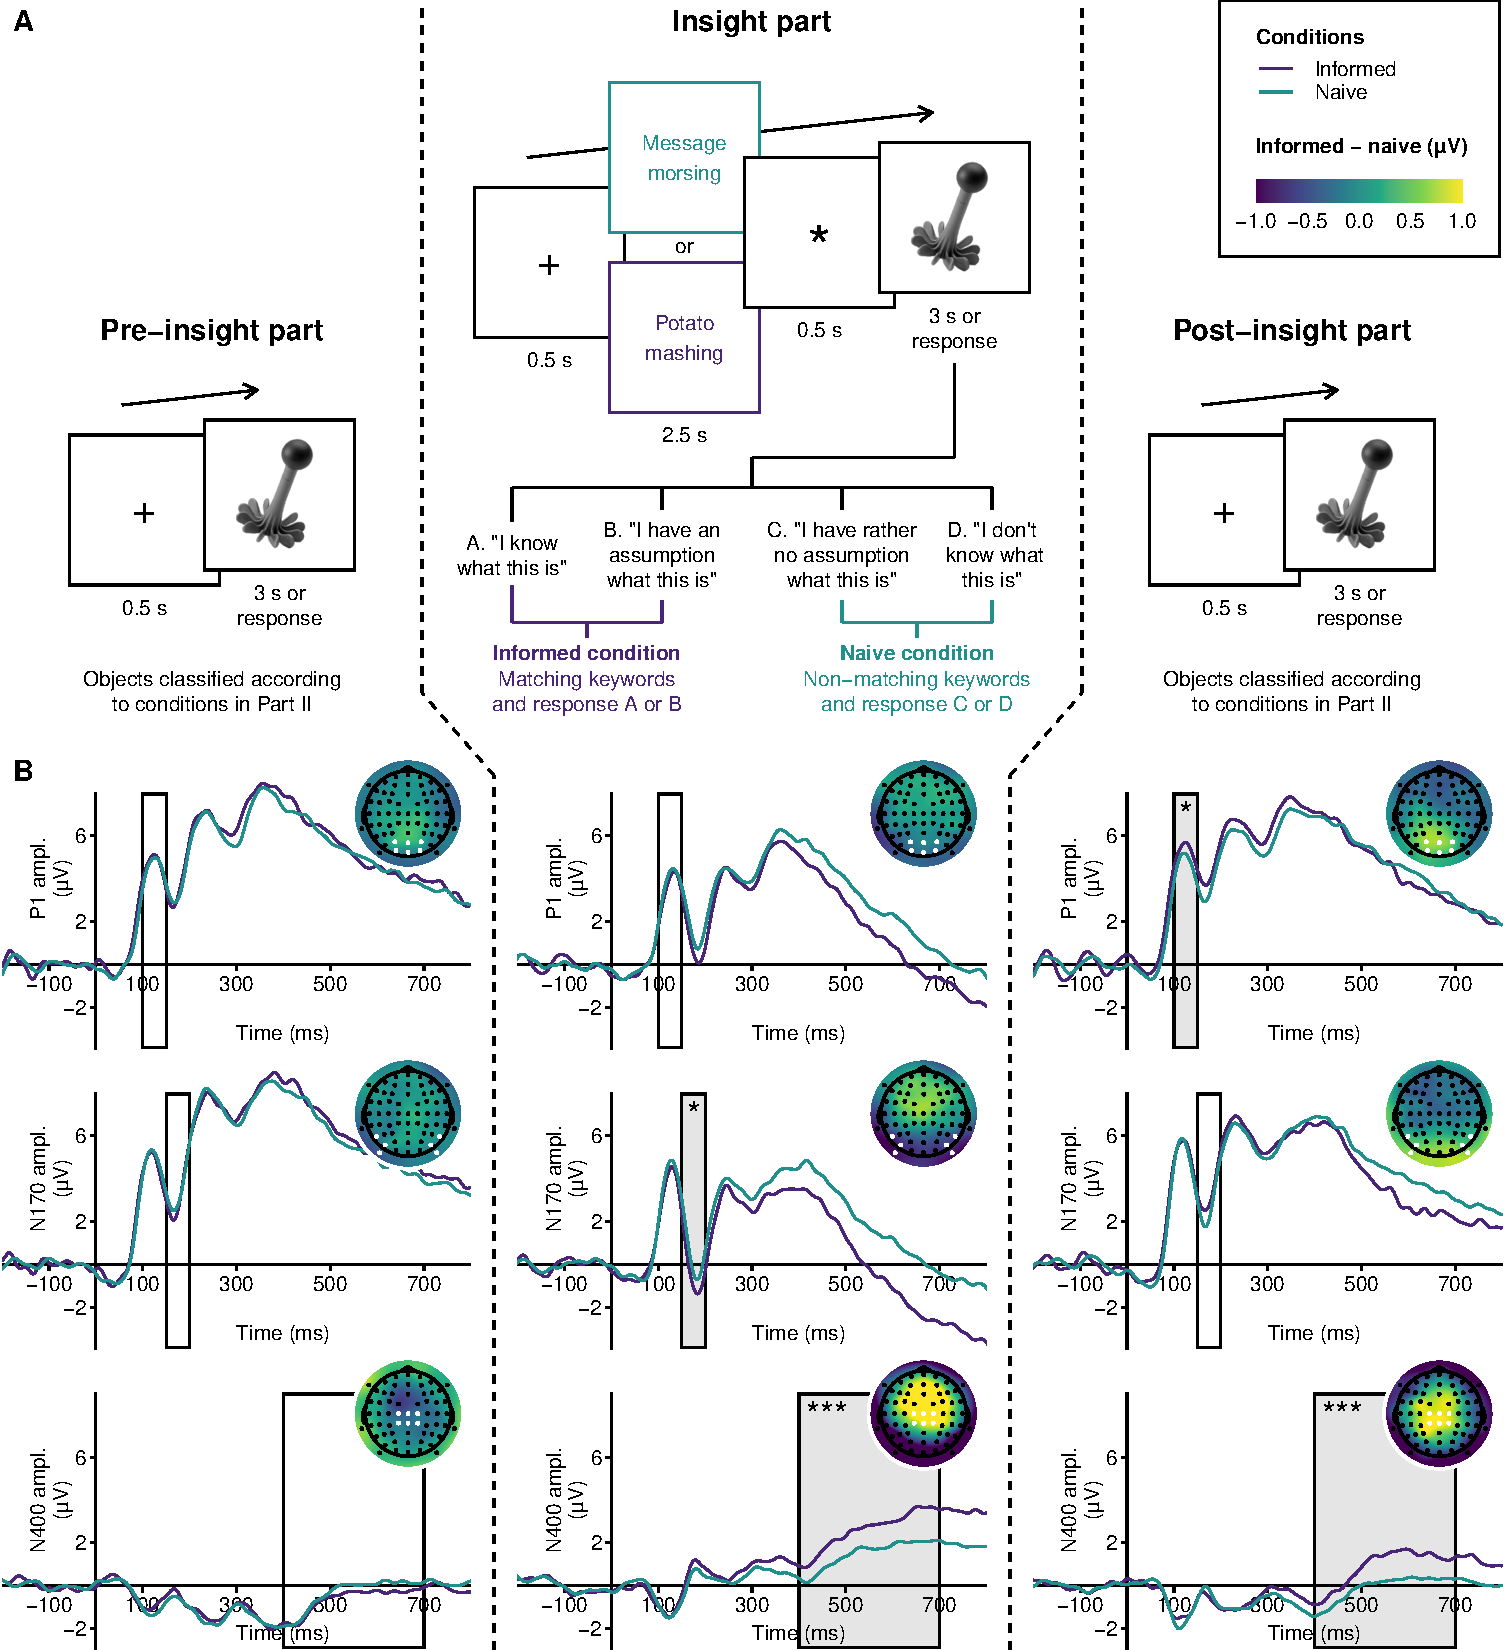
\includegraphics[width=1\linewidth]{manuscript_files/figure-latex/exp1-plot-1} 

}

\caption{Procedure and results of Experiment 1. \emph{(A)} In the pre-insight part (Part I), participants were presented with 120 unfamiliar objects and indicated whether they knew what kind of object they were viewing. In the insight part (Part II), half of these objects were presented with matching keywords (in purple color for illustration), leading to semantically informed perception, and the other half with non-matching keywords (in petrol color for illustration), leading to naive perception. In the post-insight part (Part III), the same objects were presented again without the keywords. \emph{(B)} ERP waveforms and scalp topographies are shown for objects with semantically informed versus naive perception within Parts I, II, and III. Semantically informed perception was associated with significantly more negative amplitudes in the N170 component in Part II, significantly less negative amplitudes in the N400 component in Parts II and III, and significantly more positive amplitudes in the P1 component in Part III. Ampl. = amplitude.\newline*\emph{p} \textless{} .05. **\emph{p} \textless{} .01. ***\emph{p} \textless{} .001.}\label{fig:exp1-plot}
\end{figure}

In the \emph{insight} part (Part II), only the 120 unfamiliar objects were presented for a second time, now preceded either by matching keywords (leading to semantically informed perception) or by non-matching keywords (leading to naive perception). Each trial consisted of a fixation cross presented for 0.5 s, followed by the presentation of the keywords for 2.5 s. Then, an asterisk was presented in the middle of the screen for another 0.5 s, followed by the presentation of the object until a response was made or until a time out after 3 s. The objects were presented in blocks of 30 trials so that within each block (a) there were 15 objects from each of the two experimental conditions and (b) objects were heterogeneous in terms of their shape, visual complexity, and functional category (e.g.~medical devices, musical instruments).

In the post-insight part (Part III), the unfamiliar objects were presented for a third time with an identical trial structure as in Part I, i.e.~without any keywords. Note that Parts II and III were presented in an interleaved fashion so that after the presentation of one block of 30 objects in Part II (with keywords), participants took a self-timed break and continued with the same block of 30 objects in Part III (without keywords) before moving on to the next block consisting of 30 different objects. They continued like this until all four blocks were completed in both Parts II and III. In total, the experiment consisted of 480 trials (120 familiar objects in Part I and 120 unfamiliar objects in Parts I, II, and III) and took participants approximately 35 minutes to complete.

\hypertarget{eeg-recording-and-preprocessing}{%
\subsubsection{EEG Recording and Preprocessing}\label{eeg-recording-and-preprocessing}}

The continuous EEG was recorded from 62 Ag/AgCl scalp electrodes placed according to the extended 10--20 system (American Electroencephalographic Society, 1991) and referenced online to an external electrode placed on the left mastoid (M1). Two additional external electrodes were placed on the right mastoid (M2) and below the left eye (IO1), respectively. During the recording, electrode impedance was kept below 5 kΩ. An online band-pass filter with a high-pass time-constant of 10 s (0.016 Hz) and a low-pass cutoff frequency of 1,000 Hz was applied before digitizing the signal at a sampling rate of 500 Hz.

Offline, the data were preprocessed using the MNE software (Version 0.21.0; Gramfort et al., 2013) in Python (Version 3.8.5; van Rossum \& Drake, 2009). First, all scalp electrodes were re-referenced to the common average. Next, artifacts resulting from blinks and eye movements were removed using independent component analysis (ICA). The first 15 components were extracted by the FastICA algorithm (Hyvärinen, 1999) after temporarily low-pass filtering the data at 1 Hz. Those components showing substantive correlations with either of two virtual EOG channels (VEOG: IO1 minus Fp1, HEOG: F9 minus F10) were removed automatically using the \emph{find\_bads\_eog} function. After artifact correction, a zero-phase, non-causal FIR filter with a lower pass-band edge at 0.1 Hz (transition bandwidth: 0.1 Hz) and an upper pass-band edge at 30 Hz (transition bandwidth: 7.5 Hz) was applied. Next, the continuous EEG was epoched into segments of 2,000 ms, starting 500 ms before the onset of the visual presentation of each unfamiliar object. The epochs were baseline-corrected by subtracting the average voltage during the 200 ms before stimulus onset. Epochs containing artifacts despite ICA, defined as peak-to-peak amplitudes exceeding 200 µV, were removed from further analysis. This led to the exclusion of an average of 2.4 trials (0.7\%) per participant (range 0 to 24). Single-trial event-related potentials were computed as the mean amplitude across time windows and regions of interests (ROIs) defined a priori, namely 100--150 ms after object onset at electrodes PO3, PO4, POz, O1, O2, and Oz for the P1 component, 150--200 ms after object onset at electrodes P7, P8, PO7, PO8, PO9, and PO10 for the N170 component, and 400--700 ms at electrodes C1, C2, Cz, CP1, CP2, and CPz for the N400 component.

\hypertarget{statistical-analysis}{%
\subsubsection{Statistical Analysis}\label{statistical-analysis}}

First, because we were interested in the effects of knowledge on perceiving \emph{unfamiliar} objects only, we excluded from all furthere analyses those objects which participants classified as being known to them in Part I (i.e.~before any keywords were presented), which led to the exclusion of an average of 7.5 objects per participant (6.3\%). Next, to clearly delineate semantically informed and naive perception, the assignment of all other objects to one of these two conditions for statistical analyses was co-determined by our experimental manipulation (matching versus non-matching keywords in Part II) and the behavioral responses of the participants themselves (Figure 1A). Objects were assigned to the semantically informed condition only if they were presented with matching keywords \emph{and} if participants indicated knowing what the object was or having an assumption. This was the case for an average of 27.0 objects per participant (44.9\% of objects presented with matching keywords). Complementarily, objects were assigned to the naive condition only if they were presented with non-matching keywords \emph{and} if participants indicated not knowing what the object was or having rather no assumption. This was the case for an average of 48.8 objects per participant (81.2\% of objects presented with non-matching keywords). Although the assignment was purely based on the manipulation and responses in Part II, when insight was thought to occurr, the same assignment was used to analyze the data from the other two parts. This allowed us to test on the one hand if the objects from both conditions differed in important aspects even before any keywords were presented (in Part I), and on the other hand if the semantic understanding acquired in Part II had any lasting effects on a subsequent, third presentation of the objects (in Part III).

The event-related potentials in response to objects from both conditions and all three parts were analyzed on the single trial level using linear mixed-effects regression models (Baayen et al., 2008; Frömer et al., 2018). For the purpose of the present study, these models have at least two desirable properties compared to more traditional approaches, such as analyses of variance (ANOVAs) performed on by-participant grand averages. First, they can account simultaneously for the non-independence of data points coming from the same participant or from the same item, whereas the neglect of the item as a random variable in ANOVAs leads to anti-conservative test statistics and strictly does not allow for inferences beyond the stimulus set under study (Bürki et al., 2018; Judd et al., 2012). Second, they can flexibly deal with unbalanced designs in which the number of trials differs across (combinations of) conditions, which is inevitable in designs where the assignment of trials to conditions is (co-)determined by the responses of the participants rather than by the experimental manipulation alone (e.g.~Fröber et al., 2017).

Three separate models were computed predicting P1, N170, and N400 mean amplitudes, respectively. All models included three fixed effects: (a) the part of the experiment, coded as a repeated contrast (i.e.~subtracting Part I from Part II and Part II from Part III, the intercept being the grand mean across all three parts), (b) the condition of the object, coded as a scaled sum contrast (i.e.~subtracting the naive from the semantically informed condition, the intercept being the grand mean across both conditions), and (c) the two-way interaction of part and condition. For details on these and other contrast coding schemes in linear (mixed-effects) models, please refer to (Schad et al., 2020). To determine the random effects structure, we always started with a maximal model containing by-participant and by-item random intercepts and random slopes for all fixed effects (Barr et al., 2013). We then performed a model selection algorithm as proposed by (Matuschek et al., 2017) in order to increase statistical power and avoid overparameterization: Iteratively, each random effects was removed and the resulting, more parsimonious model was compared to the previous, more complex model by means of a likelihood ratio test. Only if the parsimonious model explained the data equally well as the complex model (determined by \emph{p} \textgreater{} .20; Matuschek et al., 2017) did we leave the random effect out, otherwise it was kept in the final model. All models were calculated in R (Version 4.0.2; R Core Team, 2020) using the lme4 package (Version 1.1.23; Bates et al., 2015). The optimizer function \emph{bobyqa} with 2·10\textsuperscript{5} iterations was used for maximum likelihood estimation. The model selection algorithm via likelihood ratio tests was performed using the buildmer package (Version 1.7.1; Voeten, 2020). Finally, to answer our research question of whether or not semantically informed perception had an influence on the ERP components within each part, planned follow-up comparisons were calculated, contrasting the informed against the naive condition within Parts I, II, and III. All \emph{p} values subsequently reported were computed by approximating the relevant denominator degrees of freedom using Satterthwaite's methods as implemented in the lmerTest package (Kuznetsova et al., 2017).

The materials, single trial behavioral and ERP data, and all code for data analysis can be accessed via the Open Science Framework (\href{https://osf.io/myprojects/}{https://osf.io/\ldots/}). To avoid potential misuse, the raw EEG are only made available by the corresponding author upon request.

\hypertarget{results}{%
\subsection{Results}\label{results}}

Single-trial ERPs were analyzed in response to unfamiliar objects before (Part I), while (Part II), and after (Part III) participants obtained relevant semantic information about their function. Only in Part II, half of the objects were preceded by a matching description, fostering semantically informed perception to occur, whereas the other half were preceded by a non-matching description, leading to naive perception of the object. The objects were analyzed according to this manipulation in combination with participants' self-report in Part II (Figure 1A), thus making sure that semantically informed (or naive) perception did indeed occur. The analysis focused on differences between these two conditions in the P1 component (100--150 ms) as an index of lower-level visual perception, in the N170 component (150--200 ms) as index of higher-level visual perception, and in the N400 component (400--700 ms) as an index of semantic processing.

\begin{table}[tbp]

\begin{center}
\begin{threeparttable}

\caption{\label{tab:exp1-table}Results of linear mixed-effects regression models for Experiment 1}

\footnotesize{

\begin{tabular}{lcccccc}
\toprule
 & \multicolumn{2}{c}{\textbf{P1}} & \multicolumn{2}{c}{\textbf{N170}} & \multicolumn{2}{c}{\textbf{N400}} \\
\cmidrule(r){2-3} \cmidrule(r){4-5} \cmidrule(r){6-7}
\textit{Fixed effects} & \textit{F} (\textit{df}) & \textit{p} & \textit{F} (\textit{df}) & \textit{p} & \textit{F} (\textit{df}) & \textit{p}\\
\midrule
Part & 10.89 (2, 24.5) & < .001 & 14.18 (2, 24.9) & < .001 & 32.85 (2, 25.6) & < .001\\
Condition & 0.60 (1, 5343.5) & .438 & 0.30 (1, 24.2) & .586 & 13.00 (1, 24.4) & .001\\
Pt. × con. & 2.30 (2, 4605.0) & .100 & 4.84 (2, 4878.2) & .008 & 10.91 (2, 5120.9) & < .001\\
\textit{Informed $-$  naive} & Est. [95\% CI] & \textit{p} & Est. [95\% CI] & \textit{p} & Est. [95\% CI] & \textit{p}\\ \midrule
Part I (pre-insight) & -0.03 [-0.53, 0.47] & .913 & -0.12 [-0.68, 0.44] & .665 & -0.20 [-0.65, 0.26] & .400\\
Part II (insight) & -0.18 [-0.68, 0.32] & .490 & -0.64 [-1.20, -0.08] & .026 & 0.93 [0.48, 1.39] & < .001\\
Part II (post-insight) & 0.55 [0.05, 1.05] & .031 & 0.43 [-0.14, 0.99] & .136 & 1.00 [0.54, 1.46] & < .001\\
\bottomrule
\addlinespace
\end{tabular}

}

\begin{tablenotes}[para]
\normalsize{\textit{Note.} Pt. = part, con. = condition, est. = estimate, CI = confidence interval.}
\end{tablenotes}

\end{threeparttable}
\end{center}

\end{table}

Averaged across conditions, P1, N170, and N400 amplitudes differed as a function of the part of the experiment, all \emph{F}s \textgreater{} 10.89, all \emph{p}s \textless{} .001 (Table \ref{tab:exp1-table}). In addition, N400 amplitudes differed between the informed and the naive condition averaged across the three parts of the experiment, \emph{F}NA = NA, \emph{p} = NA. Crucially, the part × condition interaction was significant in the N170 component, \emph{F}(2, 4878.2) = 4.84, \emph{p} = .008, and in the N400 component, \emph{F}(2, 5120.9) = 10.91, \emph{p} \textless{} .001, while also being marginally significant in the P1 component, \emph{F}(2, 4605.0) = 2.30, \emph{p} = .100. To answer our main research question, we decomposed these interactions into the differences between the semantically informed condition and the naive condition within the three different parts of the experiment.

\hypertarget{erps-in-part-i-pre-insight}{%
\subsubsection{ERPs in Part I (Pre-Insight)}\label{erps-in-part-i-pre-insight}}

In Part I, when objects were unfamiliar to the participant and presented without keywords, no differences emerged between the semantically informed and the naive condition in the P1, N170, or N400 component, all \emph{p}s \textgreater{} .400 (Table \ref{tab:exp1-table}, Figure \ref{fig:exp1-plot}B \& C). On the one hand, this was to be expected given that the critical presentation of the keywords (leading to semantically informed vs.~naive perception) had not yet taken place. On the other hand, the absence of reliable differences in Part I can be taken as evidence---with the usual caveats when interpreting null effects---that any subsequent effect of the semantic information in Parts II and III cannot be accounted for by visual differences between the objects in the two conditions. Although the presentation of a matching or non-matching keywords for each object was counterbalanced across participants, the fact that different numbers of objects were assigned to the two conditions based on participants' self report in Part II would have made it possible for such visual differences to emerge as a confounding factor. If they did, however, one would expect to detect these differences even before any keywords were presented, which we have now seen was not the case.

\hypertarget{erps-in-part-ii-insight}{%
\subsubsection{ERPs in Part II (Insight)}\label{erps-in-part-ii-insight}}

In Part II, half of the unfamiliar objects were presented with matching keywords (for forming the semantically informed condition) and the other half were presented with non-matching keywords (for forming the naive condition). When semantic information informed the perception of the object (akin to an insight experience), the amplitude of the N170 component was significantly enlarged (i.e.~more negative), \emph{b} = -0.64 µV, \emph{p} = .026, and the amplitude of the N400 component was significantly reduced (i.e.~less negative), \emph{b} = 0.93 µV, \emph{p} \textless{} .001, compared to when an object was viewed naively without relevant semantic information. As in Part I, there were no reliable differences in the P1 component, \emph{p} = .490.

\hypertarget{erps-in-part-iii-post-insight}{%
\subsubsection{ERPs in Part III (Post-Insight)}\label{erps-in-part-iii-post-insight}}

In Part III, the unfamiliar objects were presented for a third time, again without the keywords (as in Part I), to test whether the semantic information had any lasting effects on the processing of the objects. As in Part II, the N400 component remained significantly reduced during semantically informed as compared to naive perception, \emph{b} = 1.00 µV, \emph{p} \textless{} .001, whereas the early effect in the N170 component did not reoccur, \emph{p} = .136. Instead, we now observed an even earlier modulation in the P1 component, which was significantly enlarged (i.e.~more positive) in response to objects for which semantically informed perception had taken place, \emph{b} = 0.55 µV, \emph{p} = .031.

\hypertarget{discussion}{%
\subsection{Discussion}\label{discussion}}

In Experiment 1, we measured event-related brain potentials from participants viewing unfamiliar objects before (Part I), while (Part II) and after (Part III) they were able to understand what kind of object they saw. To induce this semantically informed perception, half of the objects in Part II were preceded by matching verbal keywords about their typical function or use, whereas the other half were preceded by non-matching keywords, serving as a naive baseline condition.

Participants' semantically informed perception of the objects in Part II was associated with a significantly enlarged N170 component, indicating that the sudden acquisition of knowledge about the object influenced aspects of its higher-level visual processing (Rossion \& Jacques, 2011; Tanaka \& Curran, 2001). The fact that this effect did not reoccur in Part III, when the objects were presented once more without keywords, suggests it being a marker of insight through semantic information that is altering object processing online. In contrast, we also observed a modulation of the N400 component, which was reduced for objects while insight was taking place (in Part II) and remained so when the same objects were presented repeatedly (in Part III). The N400 is most often discussed as an index of increased demands for semantic processing or integration (Kutas \& Federmeier, 2011; Lau et al., 2008; Rabovsky et al., 2018). Its reduction can thus be interpreted as lowered semantic processing demands in response to unfamiliar objects once participants had understood what kind of object they were viewing. Finally, semantically informed perception was also associated with increased amplitudes in the P1 component, but only once the objects were presented for a third time (in Part III), after the critical presentation during which insight had occurred (in Part II). This effect, which replicates previous work on obtaining knowledge about previously unfamiliar images (e.g.~Samaha et al., 2018), may be associated with the newly acquired semantic knowledge exerting an influence on lower-level visual perception, either online or through altered visual representations of the objects for which insight had occurred.

Because of the exploratory nature of the present study and the novelty of the ERP effects observed in Experiment 1, we ran a replication study to assess the robustness of these findings in another samples of participants.

\hypertarget{experiment-2}{%
\section{Experiment 2}\label{experiment-2}}

\hypertarget{methods-1}{%
\subsection{Methods}\label{methods-1}}

\hypertarget{participants-1}{%
\subsubsection{Participants}\label{participants-1}}

Participants for Experiment 2 were 24 German native speakers (15 female, 9 male) with a mean age of 26 years (range 19 to 29) who had not participated in Experiment 1. They had no history of psychological disorder or treatment, were right-handed and reported normal or corrected-to-normal vision. They gave written informed consent before starting the experiment and received a compensation of €8 per hour for participating.

\hypertarget{materials-procedure-and-analysis}{%
\subsubsection{Materials, Procedure, and Analysis}\label{materials-procedure-and-analysis}}

All materials, procedures, EEG-related methods, and statistical analyses were identical to Experiment 1. An average of 7.0 objects per participant (5.8\%) was classified as being known in Part I and excluded from all further analyses. Based on participants' responses in Part II, an average of 26.4 objects were assigned to the semantically informed condition (44.0\% of objects presented with matching keywords) and an average of 49.2 objects were assigned to the naive condition (82.0\% of objects presented with a non-matching description). Automatic rejection of EEG epochs containing artifacts led to the exclusion of 11.0 trials per participant (3.0\%, range 0 to 85).

\hypertarget{results-1}{%
\subsection{Results}\label{results-1}}

\begin{table}[tbp]

\begin{center}
\begin{threeparttable}

\caption{\label{tab:exp2-table}Results of linear mixed-effects regression models for Experiment 2}

\footnotesize{

\begin{tabular}{lcccccc}
\toprule
 & \multicolumn{2}{c}{\textbf{P1}} & \multicolumn{2}{c}{\textbf{N170}} & \multicolumn{2}{c}{\textbf{N400}} \\
\cmidrule(r){2-3} \cmidrule(r){4-5} \cmidrule(r){6-7}
\textit{Fixed effects} & \textit{F} (\textit{df}) & \textit{p} & \textit{F} (\textit{df}) & \textit{p} & \textit{F} (\textit{df}) & \textit{p}\\
\midrule
Part & 17.45 (2, 5267.1) & < .001 & 16.57 (2, 25.1) & < .001 & 70.12 (2, 25.2) & < .001\\
Condition & 0.02 (1, 5276.9) & .900 & 0.98 (1, 5228.5) & .322 & 19.95 (1, 5242.5) & < .001\\
Pt. × con. & 3.60 (2, 5267.1) & .027 & 1.25 (2, 4756.5) & .287 & 7.92 (2, 4714.9) & < .001\\
\textit{Informed $-$  naive} & Est. [95\% CI] & \textit{p} & Est. [95\% CI] & \textit{p} & Est. [95\% CI] & \textit{p}\\ \midrule
Part I (pre-insight) & -0.16 [-0.71, 0.40] & .582 & -0.03 [-0.53, 0.48] & .920 & 0.04 [-0.43, 0.50] & .877\\
Part II (insight) & -0.48 [-1.03, 0.08] & .094 & -0.48 [-0.99, 0.03] & .064 & 1.33 [0.87, 1.79] & < .001\\
Part II (post-insight) & 0.57 [0.01, 1.13] & .047 & 0.06 [-0.45, 0.57] & .818 & 0.47 [0.01, 0.93] & .047\\
\bottomrule
\addlinespace
\end{tabular}

}

\begin{tablenotes}[para]
\normalsize{\textit{Note.} Pt. = part, con. = condition, est. = estimate, CI = confidence interval.}
\end{tablenotes}

\end{threeparttable}
\end{center}

\end{table}

As in Experiment 1, P1, N170, and N400 amplitudes differed between the three different parts of the experiments, all \emph{F}s \textgreater{} 16.57, all \emph{p}s \textless{} .001 (Table \ref{tab:exp2-table}). Also as in Experiment 1, N400 amplitudes differed between the informed and the naive condition averaged across parts, \emph{F}NA = NA, \emph{p} NA. The part × condition interaction was significant in the P1 component, \emph{F}(2, 5267.1) = 3.60, \emph{p} = .027, and in the N400 component, \emph{F}(2, 4714.9) = 7.92, \emph{p} \textless{} .001, but not in the N170 component, \emph{F}(2, 4756.5) = 1.25, \emph{p} = .287.



\begin{figure}

{\centering 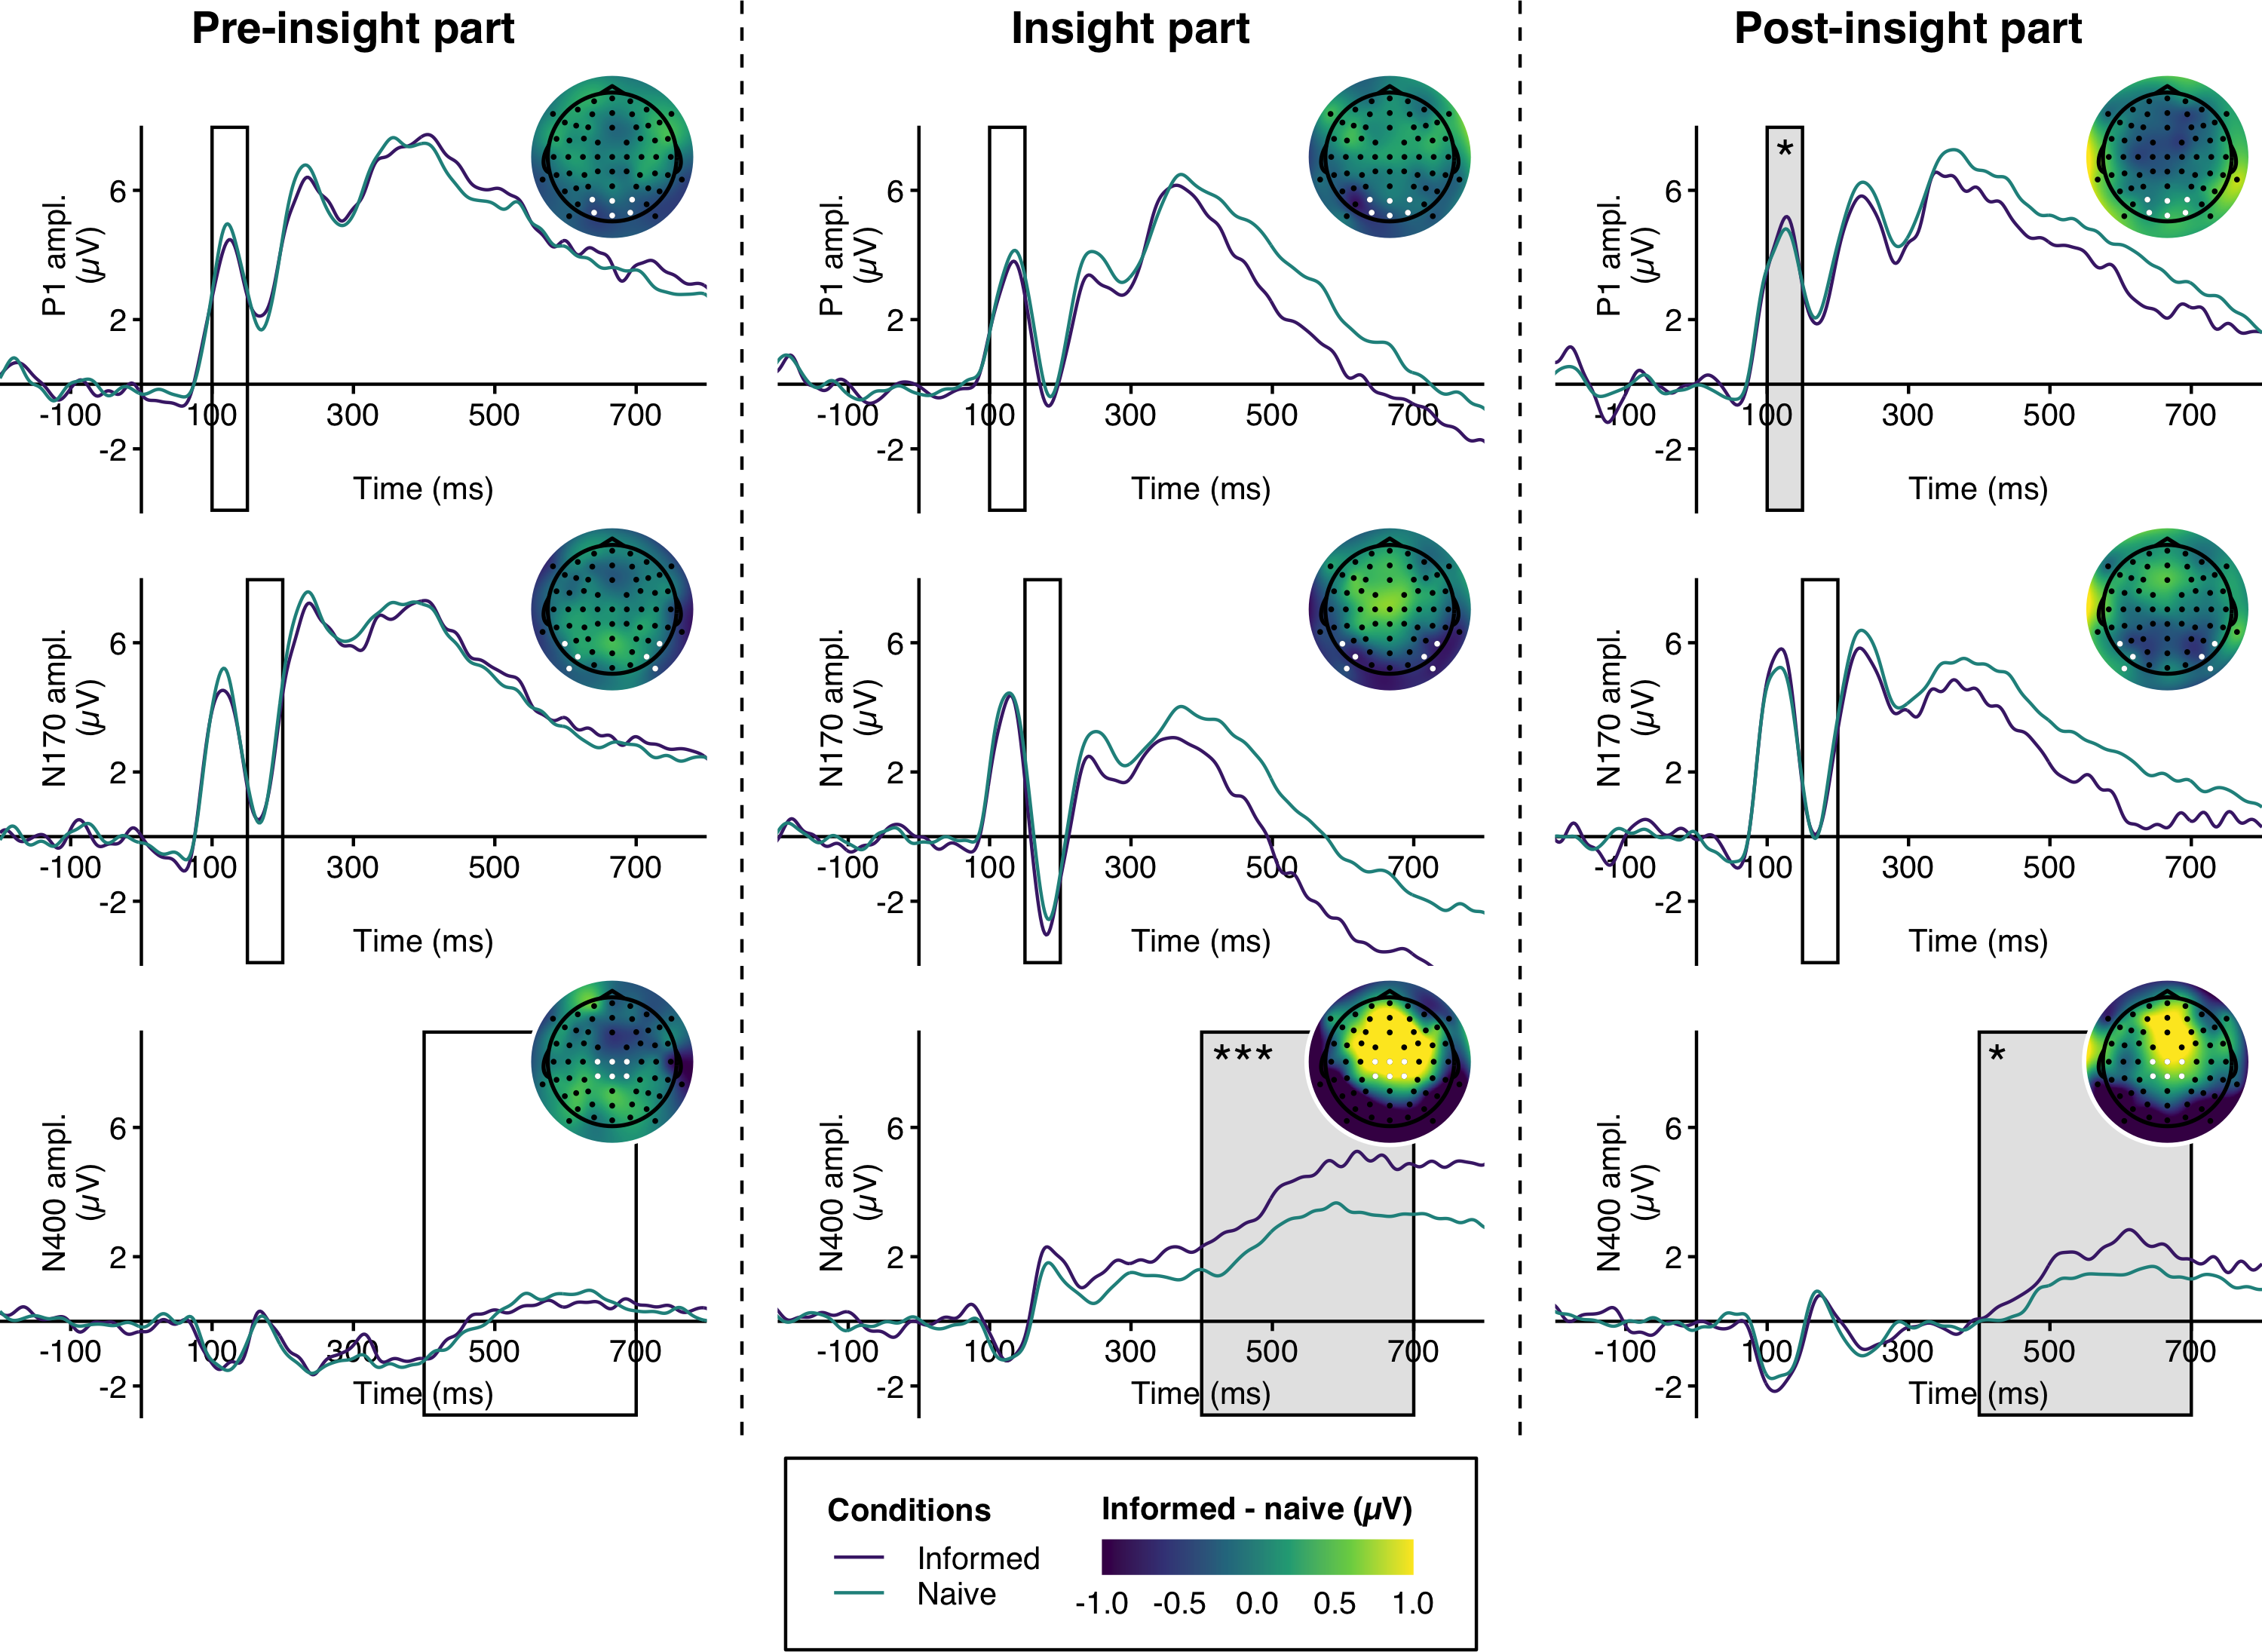
\includegraphics[width=1\linewidth]{manuscript_files/figure-latex/exp2-plot-1} 

}

\caption{Results of Experiment 2. ERP waveforms and scalp topographies are shown for objects for which participants experienced semantically informed versus naive perception within Parts I, II, and III. In a direct replication of Experiment 1, the effect of semantic information on the N400 component in Parts II and III and on the P1 component in Part III remained statistically significant, while the effect on the N170 component in Part II remained only marginally significant (\emph{p} = .064). Ampl. = amplitude.\newline*\emph{p} \textless{} .05. **\emph{p} \textless{} .01. ***\emph{p} \textless{} .001.}\label{fig:exp2-plot}
\end{figure}

\hypertarget{erps-in-part-i-pre-insight-1}{%
\subsubsection{ERPs in Part I (Pre-Insight)}\label{erps-in-part-i-pre-insight-1}}

As in Experiment 1, no differences between objects in the semantically informed and the naive condition emerged in the P1, N170, or N400 component, all \emph{p}s \textgreater{} .582 (Table \ref{tab:exp2-table}, Figure \ref{fig:exp2-plot}).

\hypertarget{erps-in-part-ii-insight-1}{%
\subsubsection{ERPs in Part II (Insight)}\label{erps-in-part-ii-insight-1}}

As in Experiment 1, semantically informed as compared to naive perception (induced by matching versus non-matching keywords) was associated with a (marginally) significant enhancement of the N170 component, \emph{b} = -0.48 µV, \emph{p} = .064, and a significant reduction of the N400 component, \emph{b} = 0.93 µV, \emph{p} \textless{} .001.

\hypertarget{erps-in-part-iii-post-insight-1}{%
\subsubsection{ERPs in Part III (Post-Insight)}\label{erps-in-part-iii-post-insight-1}}

As in Experiment 1, the presentation of the same unfamiliar objects for a third time (without keywords, as in Part I) led to significantly larger amplitudes in the P1 component in response to objects for which semantically informed perception had occurred, \emph{b} = 0.57 µV, \emph{p} = .047. Also, N400 amplitudes in response to these objects remained significantly reduced, \emph{b} = 0.47 µV, \emph{p} = .047.

\hypertarget{joint-analysis-of-experiments-1-and-2}{%
\subsubsection{Joint Analysis of Experiments 1 and 2}\label{joint-analysis-of-experiments-1-and-2}}

In an attempt to maximize statistical power, we combined the ERP data sets from Experiments 1 and 2. This allowed us to determine (a) if the above effects---including the marginally significant ones---were reliable when tested in a larger sample, and (b) if there were significant differences in the ERP amplitudes between Experiments 1 and 2. Methods for statistical analysis were kept unchanged apart from the addition of a new factor denoting the experiment, coded as a scaled sum contrast (i.e.~subtracting Experiment 1 from Experiment 2, the intercept being the grand mean across both experiments; Schad et al., 2020). This factor and its possible interactions with part, condition, and part × condition were included in the linear mixed-effects regression models as fixed effects and as potential by-item random slopes. They were not included as by-participant random slopes since different participants took part in Experiments 1 and 2. Note that, as above, random effects were eventually included only if their omission led to a significant decline in model fit (Matuschek et al., 2017; Voeten, 2020).

\begin{table}[tbp]

\begin{center}
\begin{threeparttable}

\caption{\label{tab:joint-table}Results of linear mixed-effects regression models for Experiments 1 and 2 combined}

\footnotesize{

\begin{tabular}{lcccccc}
\toprule
 & \multicolumn{2}{c}{\textbf{P1}} & \multicolumn{2}{c}{\textbf{N170}} & \multicolumn{2}{c}{\textbf{N400}} \\
\cmidrule(r){2-3} \cmidrule(r){4-5} \cmidrule(r){6-7}
\textit{Fixed effects} & \textit{F} (\textit{df}) & \textit{p} & \textit{F} (\textit{df}) & \textit{p} & \textit{F} (\textit{df}) & \textit{p}\\
\midrule
Part & 12.34 (2, 49.1) & < .001 & 30.08 (2, 50.3) & < .001 & 94.61 (2, 50.6) & < .001\\
Condition & 0.15 (1, 10573.1) & .699 & 1.16 (1, 45.2) & .287 & 41.38 (1, 10593.6) & < .001\\
Experiment & 0.33 (1, 48.2) & .567 & 2.50 (1, 48.0) & .121 & 4.96 (1, 48.4) & .031\\
Pt. × con. & 3.90 (2, 9004.9) & .020 & 5.26 (2, 9904.1) & .005 & 15.34 (2, 10091.0) & < .001\\
Pt. × exp. & 0.04 (2, 49.1) & .966 & 0.58 (2, 50.3) & .565 & 2.55 (2, 50.6) & .088\\
Ins. × exp. & 0.43 (1, 10573.1) & .514 & 0.06 (1, 45.2) & .805 & 0.07 (1, 10593.6) & .785\\
Pt. × con. × exp. & 0.03 (2, 9004.9) & .968 & 0.58 (2, 9904.1) & .559 & 2.54 (2, 10091.0) & .079\\
\textit{Informed $-$  naive} & Est. [95\% CI] & \textit{p} & Est. [95\% CI] & \textit{p} & Est. [95\% CI] & \textit{p}\\ \midrule
Part I (pre-insight) & -0.10 [-0.47, 0.28] & .616 & -0.10 [-0.48, 0.29] & .611 & -0.09 [-0.39, 0.22] & .577\\
Part II (insight) & -0.24 [-0.62, 0.13] & .202 & -0.57 [-0.96, -0.18] & .004 & 1.10 [0.80, 1.41] & < .001\\
Part II (post-insight) & 0.47 [0.09, 0.84] & .014 & 0.24 [-0.15, 0.63] & .225 & 0.73 [0.42, 1.04] & < .001\\
\bottomrule
\addlinespace
\end{tabular}

}

\begin{tablenotes}[para]
\normalsize{\textit{Note.} Pt. = part, con. = condition, exp. = experiment, est. = estimate, CI = confidence interval.}
\end{tablenotes}

\end{threeparttable}
\end{center}

\end{table}

As shown in Table \ref{tab:joint-table}, the main effect of the part of the experiment was significant in the P1, N170, and N400 component, all \emph{F}s \textgreater{} 12.34, all \emph{p}s \textless{} .001, as was the main effect of condition in the N400, \emph{F}NA = NA, \emph{p} NA. Furthermore, the part × condition interaction was now observed reliably in all three components, all \emph{F}s \textgreater{} 3.90, all \emph{p}s \textless{} .020. While there was a main effect of experiment in the N400, \emph{F}(1, 48.4) = 4.96, \emph{p} = .031, the absence of any significant interactions of experiment with part or condition indicated that the effects of our experimental manipulations did not differ between Experiments 1 and 2.



\begin{figure}

{\centering 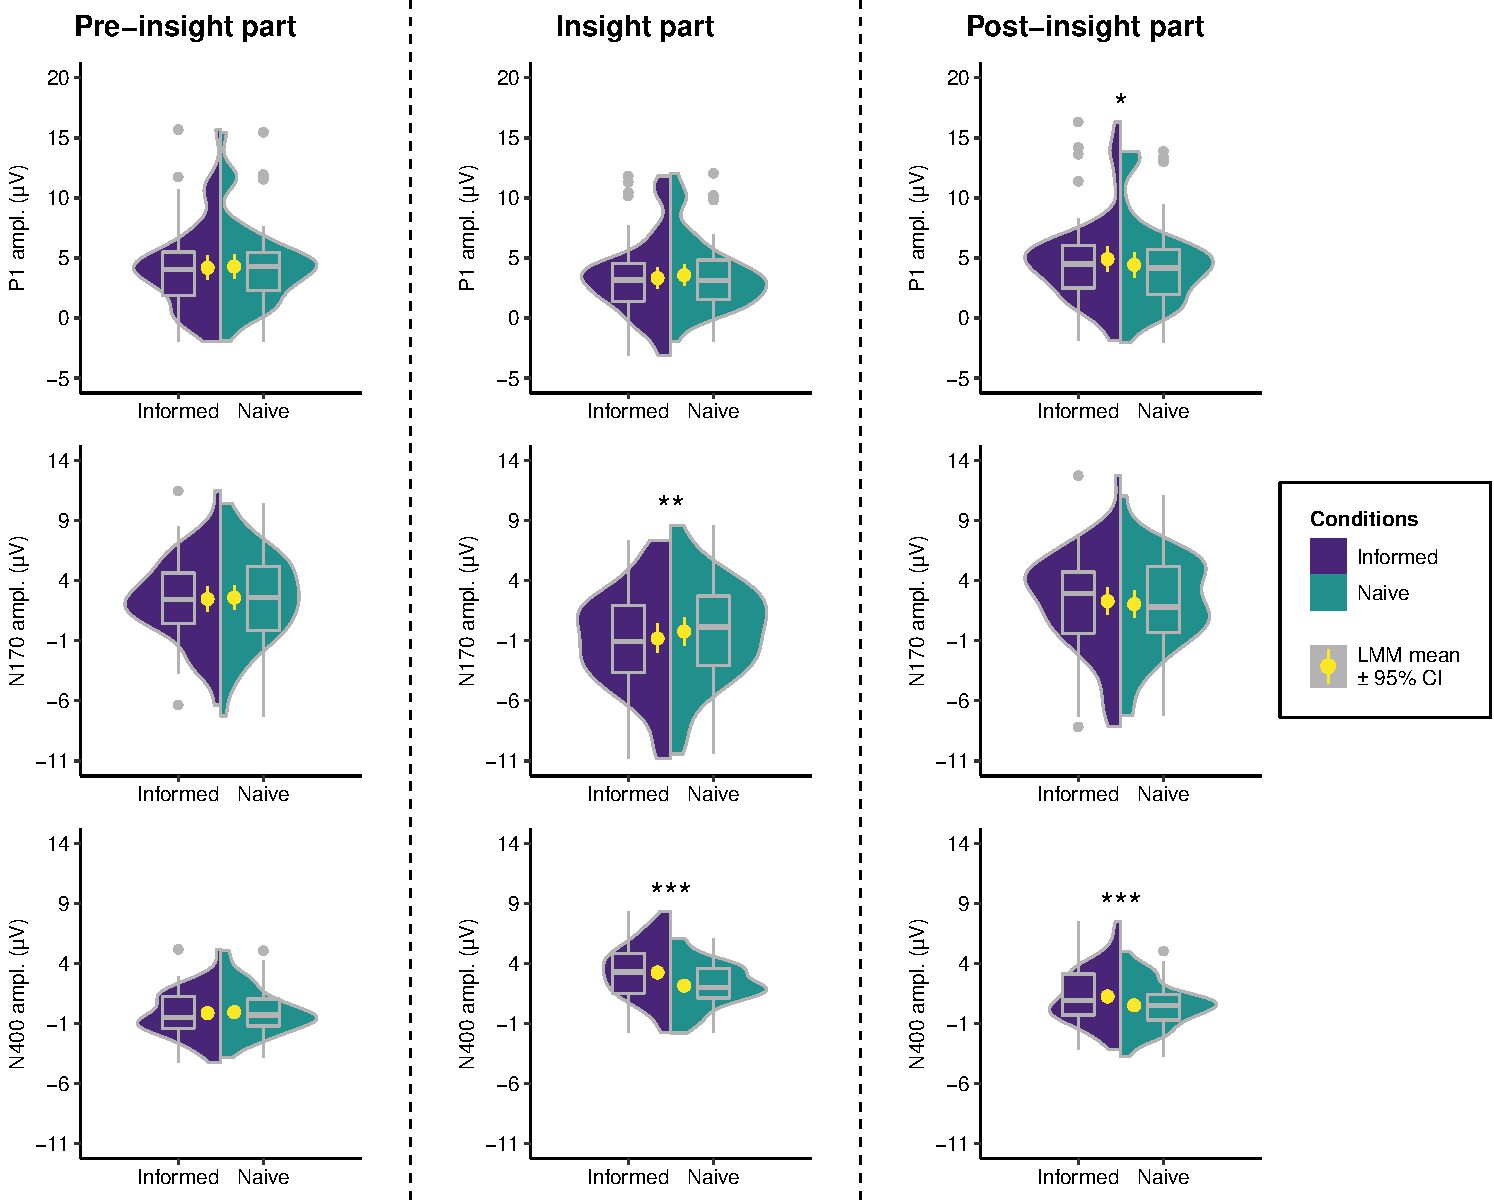
\includegraphics[width=1\linewidth]{manuscript_files/figure-latex/joint-plot-1} 

}

\caption{Measured and modelled ERP amplitudes for Experiments 1 and 2 combined. The violins and boxplots show the distributions of the by-participant grand averaged ERPs during semantically informed perception (in purple color) and naive perception (in petrol color), separately for Parts I (before insight was occurring), II (while insight was occurring), and III (after insight had occurred). The yellow dots show the corresponding condition means as predicted by linear mixed-effects modelling (see main text and Table \ref{tab:joint-table}), together with their respective 95\% confidence interval. Ampl. = amplitude, CI = confidence interval, LMM = linear mixed-effects model.\newline*\emph{p} \textless{} .05. **\emph{p} \textless{} .01. ***\emph{p} \textless{} .001.}\label{fig:joint-plot}
\end{figure}

Based on the part × condition interaction, we again computed follow-up comparisons between the semantically inforemd and the naive condition within each part, now collapsed across the data from both experiments (Figure \ref{fig:joint-plot}). This confirmed the absence of any reliable differences between the two conditions in Part I, all \emph{p}s \textgreater{} .577, the significant enhancement of the N170 component in Part II, while the semantic information was obtained, \emph{b} = -0.57 µV, \emph{p} = .004, the significant reduction of the N400 component in Part II, while the semantic information was obtained, \emph{b} = 1.10 µV, \emph{p} \textless{} .001, and Part III, after the information had been obtained, \emph{b} = 0.73 µV, \emph{p} = \textless{} .001, as well as the significant enhancement of the P1 component in Part III, after the information had been obtained, \emph{b} = 0.47 µV, \emph{p} = .014.

\hypertarget{control-analysis}{%
\subsubsection{Control Analysis}\label{control-analysis}}

One may raise concerns whether the modulation of the N170 component in Part II genuinely reflects the semantically informed perception of the objects in the respective condition, or---as an alternative explanation---whether it could be driven by the objects in the other, semantically naive condition. Remember that these objects were preceded by non-matching keywords which were picked so that they could not be related to the object's visual features and their configuration. Thus, the modulation of the ERP components in Part II may reflect a mismatch response to those objects---reflecting, for example, the fact that the visual features of the object shown in Figure \ref{fig:exp1-plot}A cannot be reconciled with the function of morsing messages. To preclude this alternative explanation, we repeated the analysis above using a different baseline against which the objects in the semantically informed condition were contrasted. Instead of the naive condition (where objects were presented with non-matching descriptions), we now used those objects which were preceded by matching descriptions (as in the informed condition), but which were excluded from the main analysis because participants indicated behaviorally that they did not understand the object they were seeing. Across both experiments, this was the case for 49.6\% of objects presented with matching descriptions as compared to 44.4\% of objects which did indeed lead to semantically informed perception.\footnote{Note that the remaining objects to make it up to 100\% were excluded as not being unfamiliar in Part I of the experiment (see Methods).} Just as above, this control analysis revealed a robust N170 effect in Part II, \emph{b} = -1.00 µV, \emph{p} \textless{} .001. Thus, this enhanced negativity seems to be a genuine marker of semantically informed perception, no matter if compared to objects presented with misleading keywords or compared to objects presented with accurate keywords on which participants failed to capitalize. Note that the reduction of the N400 component in Part II also remained robust in this control analysis, \emph{b} = 1.25 µV, \emph{p} \textless{} .001.

\hypertarget{discussion-1}{%
\subsection{Discussion}\label{discussion-1}}

Experiment 2, which was a direct replication of Experiment 1, confirmed the effects of obtaining semantic information about previously unfamiliar objects on ERPs associated with lower-level visual perception (P1), higher-level visual perception (N170), and semantic processing (N400). While the enhancement of the N170 component, being more negative for semantically informed as compared to naive perception, was present only during the critical presentation of the objects with their respective keywords (in Part II), the enhancement of the P1, being more positive in response to these same objects, emerged only after the information had been obtained and the objects were presented again (in Part III). This indicates a modulation of different stages of visual object perception through semantic knowledge, while and after an understanding of the object has been obtained. Finally, a sustained reduction of the N400 component in response to objects for which participants experienced semantically informed perception may reflect lowered semantic processing demands compared to unfamiliar objects which participants did not yet understand.

\hypertarget{general-discussion}{%
\section{General Discussion}\label{general-discussion}}

General discussion section goes here.

Although most of the previous studies in the object processing domain have focused on the P1 component as an index of semantic knowledge modulating perceptual processes, at least two studies provide evidence for top-down effects of meaningfulness on the visual N170 (or N1) component in response to schematic drawings of faces (Bentin \& Golland, 2002) and objects (Beaucousin et al., 2011). Using a similar design as in the present study, drawings of distored faces elicited a facelike (i.e.~enlarged) N170 component only after participants were primed with a vaild hint---in this case the same face with all of its visual features in place (Bentin \& Golland, 2002). Similarly, N170 amplitudes in a global-local detection task where shown to be enhanced in response to line drawings of meaningful objects (a boat or a butterfly) as compared to visually matched by meaningless drawings of non-objects. Interestingly, this effect was reversed in polarity when participants had to focus on the smaller, constituent parts and ignoring the object which emerged out of their global arrangement, which may be interpreted as further evidence for a functional role of the N170 component in the holistic perception of an object and its early visual categorization, integrating across its visual features.

\newpage

\hypertarget{references}{%
\section{References}\label{references}}

\setlength{\parindent}{-0.5in}
\setlength{\leftskip}{0.5in}

\hypertarget{refs}{}
\leavevmode\hypertarget{ref-abdelrahman2011}{}%
Abdel Rahman, R. (2011). Facing good and evil: Early brain signatures of affective biographical knowledge in face recognition. \emph{Emotion}, \emph{11}(6), 1397--1405. \url{https://doi.org/10.1037/a0024717}

\leavevmode\hypertarget{ref-abdelrahman2008}{}%
Abdel Rahman, R., \& Sommer, W. (2008). Seeing what we know and understand: How knowledge shapes perception. \emph{Psychonomic Bulletin \& Review}, \emph{15}(6), 1055--1063. \url{https://doi.org/10.3758/PBR.15.6.1055}

\leavevmode\hypertarget{ref-americanelectroencephalographicsociety1991}{}%
American Electroencephalographic Society. (1991). American Electroencephalographic Society guidelines for standard electrode position nomenclature. \emph{Journal of Clinical Neurophysiology}, \emph{8}(2), 200--202.

\leavevmode\hypertarget{ref-baayen2008}{}%
Baayen, R. H., Davidson, D. J., \& Bates, D. M. (2008). Mixed-effects modeling with crossed random effects for subjects and items. \emph{Journal of Memory and Language}, \emph{59}(4), 390--412. \url{https://doi.org/10.1016/j.jml.2007.12.005}

\leavevmode\hypertarget{ref-balcetis2010}{}%
Balcetis, E., \& Dunning, D. (2010). Wishful seeing: More desired objects are seen as closer. \emph{Psychological Science}, \emph{21}(1), 147--152. \url{https://doi.org/10.1177/0956797609356283}

\leavevmode\hypertarget{ref-barr2013}{}%
Barr, D. J., Levy, R., Scheepers, C., \& Tily, H. J. (2013). Random effects structure for confirmatory hypothesis testing: Keep it maximal. \emph{Journal of Memory and Language}, \emph{68}(3), 255--278. \url{https://doi.org/10.1016/j.jml.2012.11.001}

\leavevmode\hypertarget{ref-R-lme4}{}%
Bates, D., Mächler, M., Bolker, B., \& Walker, S. (2015). Fitting linear mixed-effects models using lme4. \emph{Journal of Statistical Software}, \emph{67}(1), 1--48. \url{https://doi.org/10.18637/jss.v067.i01}

\leavevmode\hypertarget{ref-beaucousin2011}{}%
Beaucousin, V., Cassotti, M., Simon, G., Pineau, A., Kostova, M., Houdé, O., \& Poirel, N. (2011). ERP evidence of a meaningfulness impact on visual global/local processing: When meaning captures attention. \emph{Neuropsychologia}, \emph{49}(5), 1258--1266. \url{https://doi.org/10.1016/j.neuropsychologia.2011.01.039}

\leavevmode\hypertarget{ref-bentin1996}{}%
Bentin, S., Allison, T., Puce, A., Perez, E., \& McCarthy, G. (1996). Electrophysiological studies of face perception in humans. \emph{Journal of Cognitive Neuroscience}, \emph{8}(6), 551--565. \url{https://doi.org/10.1162/jocn.1996.8.6.551}

\leavevmode\hypertarget{ref-bentin2002}{}%
Bentin, S., \& Golland, Y. (2002). Meaningful processing of meaningless stimuli: The influence of perceptual experience on early visual processing of faces. \emph{Cognition}, \emph{86}(1), B1--B14. \url{https://doi.org/10.1016/S0010-0277(02)00124-5}

\leavevmode\hypertarget{ref-bocanegra2009}{}%
Bocanegra, B. R., \& Zeelenberg, R. (2009). Emotion improves and impairs early vision. \emph{Psychological Science}, \emph{20}(6), 707--713. \url{https://doi.org/10.1111/j.1467-9280.2009.02354.x}

\leavevmode\hypertarget{ref-boutonnet2015}{}%
Boutonnet, B., \& Lupyan, G. (2015). Words jump-start vision: A label advantage in object recognition. \emph{Journal of Neuroscience}, \emph{35}(25), 9329--9335. \url{https://doi.org/10.1523/JNEUROSCI.5111-14.2015}

\leavevmode\hypertarget{ref-buxfcrki2018}{}%
Bürki, A., Frossard, J., \& Renaud, O. (2018). Accounting for stimulus and participant effects in event-related potential analyses to increase the replicability of studies. \emph{Journal of Neuroscience Methods}, \emph{309}, 218--227. \url{https://doi.org/10.1016/j.jneumeth.2018.09.016}

\leavevmode\hypertarget{ref-churchland1988}{}%
Churchland, P. M. (1988). Perceptual plasticity and theoretical neutrality: A reply to jerry fodor. \emph{Philosophy of Science}, \emph{55}(2), 167--187. \url{https://doi.org/10.1086/289425}

\leavevmode\hypertarget{ref-churchland1994}{}%
Churchland, P. S., Ramachandran, V. S., \& Sejnowski, T. J. (1994). A critique of pure vision. In \emph{Large-scale neuronal theories of the brain} (pp. 23--60). The MIT Press.

\leavevmode\hypertarget{ref-cole2012}{}%
Cole, S., Balcetis, E., \& Dunning, D. (2012). Affective signals of threat increase perceived proximity: \emph{Psychological Science}. \url{https://doi.org/10.1177/0956797612446953}

\leavevmode\hypertarget{ref-collins2014}{}%
Collins, J. A., \& Olson, I. R. (2014). Knowledge is power: How conceptual knowledge transforms visual cognition. \emph{Psychonomic Bulletin \& Review}, \emph{21}(4), 843--860. \url{https://doi.org/10.3758/s13423-013-0564-3}

\leavevmode\hypertarget{ref-dirusso2001}{}%
Di Russo, F., Martínez, A., Sereno, M. I., Pitzalis, S., \& Hillyard, S. A. (2001). Cortical sources of the early components of the visual evoked potential. \emph{Human Brain Mapping}, \emph{15}(2), 95--111. \url{https://doi.org/10.1002/hbm.10010}

\leavevmode\hypertarget{ref-eimer2011}{}%
Eimer, M., Gosling, A., Nicholas, S., \& Kiss, M. (2011). The n170 component and its links to configural face processing: A rapid neural adaptation study. \emph{Brain Research}, \emph{1376}, 76--87. \url{https://doi.org/10.1016/j.brainres.2010.12.046}

\leavevmode\hypertarget{ref-eiserbeck2020}{}%
Eiserbeck, A., \& Abdel Rahman, R. (2020). Visual consciousness of faces in the attentional blink: Knowledge-based effects of trustworthiness dominate over appearance-based impressions. \emph{Consciousness and Cognition}, \emph{83}, 102977. \url{https://doi.org/10.1016/j.concog.2020.102977}

\leavevmode\hypertarget{ref-firestone2016}{}%
Firestone, C., \& Scholl, B. J. (2016). Cognition does not affect perception: Evaluating the evidence for ``top-down'' effects. \emph{Behavioral and Brain Sciences}, \emph{39}. \url{https://doi.org/10.1017/S0140525X15000965}

\leavevmode\hypertarget{ref-fodor1984}{}%
Fodor, J. (1984). Observation reconsidered. \emph{Philosophy of Science}, \emph{51}(1), 23--43. \url{https://doi.org/10.1086/289162}

\leavevmode\hypertarget{ref-fodor1983}{}%
Fodor, J. A. (1983). \emph{The modularity of mind}. MIT Press.

\leavevmode\hypertarget{ref-foxe2002}{}%
Foxe, J. J., \& Simpson, G. V. (2002). Flow of activation from v1 to frontal cortex in humans. \emph{Experimental Brain Research}, \emph{142}(1), 139--150. \url{https://doi.org/10.1007/s00221-001-0906-7}

\leavevmode\hypertarget{ref-fruxf6ber2017}{}%
Fröber, K., Stürmer, B., Frömer, R., \& Dreisbach, G. (2017). The role of affective evaluation in conflict adaptation: An LRP study. \emph{Brain and Cognition}, \emph{116}, 9--16. \url{https://doi.org/10.1016/j.bandc.2017.05.003}

\leavevmode\hypertarget{ref-fruxf6mer2018}{}%
Frömer, R., Maier, M., \& Abdel Rahman, R. (2018). Group-level EEG-processing pipeline for flexible single trial-based analyses including linear mixed models. \emph{Frontiers in Neuroscience}, \emph{12}. \url{https://doi.org/10.3389/fnins.2018.00048}

\leavevmode\hypertarget{ref-gauthier2003a}{}%
Gauthier, I., Curran, T., Curby, K. M., \& Collins, D. (2003). Perceptual interference supports a non-modular account of face processing. \emph{Nature Neuroscience}, \emph{6}(4), 428--432. \url{https://doi.org/10.1038/nn1029}

\leavevmode\hypertarget{ref-gauthier2003}{}%
Gauthier, I., James, T. W., Curby, K. M., \& Tarr, M. J. (2003). The influence of conceptual knowledge on visual discrimination. \emph{Cognitive Neuropsychology}, \emph{20}(3-6), 507--523. \url{https://doi.org/10.1080/02643290244000275}

\leavevmode\hypertarget{ref-gramfort2013}{}%
Gramfort, A., Luessi, M., Larson, E., Engemann, D. A., Strohmeier, D., Brodbeck, C., Goj, R., Jas, M., Brooks, T., Parkkonen, L., \& al. (2013). MEG and EEG data analysis with MNE-Python. \emph{Frontiers in Neuroscience}, \emph{7}. \url{https://doi.org/10.3389/fnins.2013.00267}

\leavevmode\hypertarget{ref-gratton2009}{}%
Gratton, C., Evans, K. M., \& Federmeier, K. D. (2009). See what I mean? An ERP study of the effect of background knowledge on novel object processing. \emph{Memory \& Cognition}, \emph{37}(3), 277--291. \url{https://doi.org/10.3758/MC.37.3.277}

\leavevmode\hypertarget{ref-haber1966}{}%
Haber, R. N. (1966). Nature of the effect of set on perception. \emph{Psychological Review}, \emph{73}(4), 335--351. \url{https://doi.org/10.1037/h0023442}

\leavevmode\hypertarget{ref-hyvuxe4rinen1999}{}%
Hyvärinen, A. (1999). Fast and robust fixed-point algorithms for independent component analysis. \emph{IEEE Transactions on Neural Networks}, \emph{10}(3), 626--634. \url{https://doi.org/10.1109/72.761722}

\leavevmode\hypertarget{ref-jacques2010}{}%
Jacques, C., \& Rossion, B. (2010). Misaligning face halves increases and delays the n170 specifically for upright faces: Implications for the nature of early face representations. \emph{Brain Research}, \emph{1318}, 96--109. \url{https://doi.org/10.1016/j.brainres.2009.12.070}

\leavevmode\hypertarget{ref-johannes1995}{}%
Johannes, S., Münte, T. F., Heinze, H. J., \& Mangun, G. R. (1995). Luminance and spatial attention effects on early visual processing. \emph{Cognitive Brain Research}, \emph{2}(3), 189--205. \url{https://doi.org/10.1016/0926-6410(95)90008-X}

\leavevmode\hypertarget{ref-judd2012}{}%
Judd, C. M., Westfall, J., \& Kenny, D. A. (2012). Treating stimuli as a random factor in social psychology: A new and comprehensive solution to a pervasive but largely ignored problem. \emph{Journal of Personality and Social Psychology}, \emph{103}(1), 54--69. \url{https://doi.org/10.1037/a0028347}

\leavevmode\hypertarget{ref-kutas2011}{}%
Kutas, M., \& Federmeier, K. D. (2011). Thirty years and counting: Finding meaning in the N400 component of the event-related brain potential (ERP). \emph{Annual Review of Psychology}, \emph{62}, 621--647. \url{https://doi.org/10.1146/annurev.psych.093008.131123}

\leavevmode\hypertarget{ref-R-lmerTest}{}%
Kuznetsova, A., Brockhoff, P. B., \& Christensen, R. H. B. (2017). lmerTest package: Tests in linear mixed effects models. \emph{Journal of Statistical Software}, \emph{82}(13), 1--26. \url{https://doi.org/10.18637/jss.v082.i13}

\leavevmode\hypertarget{ref-lau2008}{}%
Lau, E. F., Phillips, C., \& Poeppel, D. (2008). A cortical network for semantics: (De)constructing the N400. \emph{Nature Reviews Neuroscience}, \emph{9}(12), 920--933. \url{https://doi.org/10.1038/nrn2532}

\leavevmode\hypertarget{ref-lin1997}{}%
Lin, E. L., \& Murphy, G. L. (1997). Effects of background knowledge on object categorization and part detection. \emph{Journal of Experimental Psychology: Human Perception and Performance}, \emph{23}(4), 1153--1169. \url{https://doi.org/10.1037/0096-1523.23.4.1153}

\leavevmode\hypertarget{ref-luck2014}{}%
Luck, S. J. (2014). Overview of common erp components. In \emph{An introduction to the event-related potential technique} (2nd ed., pp. 71--118). MIT Press.

\leavevmode\hypertarget{ref-luck2000}{}%
Luck, S. J., Woodman, G. F., \& Vogel, E. K. (2000). Event-related potential studies of attention. \emph{Trends in Cognitive Sciences}, \emph{4}(11), 432--440. \url{https://doi.org/10.1016/S1364-6613(00)01545-X}

\leavevmode\hypertarget{ref-lupyan2012}{}%
Lupyan, G. (2012). Linguistically modulated perception and cognition: The label-feedback hypothesis. \emph{Frontiers in Psychology}, \emph{3}. \url{https://doi.org/10.3389/fpsyg.2012.00054}

\leavevmode\hypertarget{ref-lupyan2015}{}%
Lupyan, G. (2015). Cognitive penetrability of perception in the age of prediction: Predictive systems are penetrable systems. \emph{Review of Philosophy and Psychology}, \emph{6}(4), 547--569. \url{https://doi.org/10.1007/s13164-015-0253-4}

\leavevmode\hypertarget{ref-lupyan2020}{}%
Lupyan, G., Abdel Rahman, R., Boroditsky, L., \& Clark, A. (2020). Effects of language on visual perception. \emph{Trends in Cognitive Sciences}, \emph{24}(11), 930--944. \url{https://doi.org/10.1016/j.tics.2020.08.005}

\leavevmode\hypertarget{ref-machery2015}{}%
Machery, E. (2015). Cognitive penetrability: A no-progress report. In J. Zeimbekis \& A. Raftopoulos (Eds.), \emph{The cognitive penetrability of perception: New philosophical perspectives}. Oxford University Press. \url{10.1093/acprof:oso/9780198738916.003.0002}

\leavevmode\hypertarget{ref-maier2018}{}%
Maier, M., \& Abdel Rahman, R. (2018). Native language promotes access to visual consciousness. \emph{Psychological Science}, \emph{29}(11), 1757--1772. \url{https://doi.org/10.1177/0956797618782181}

\leavevmode\hypertarget{ref-maier2014}{}%
Maier, M., Glage, P., Hohlfeld, A., \& Abdel Rahman, R. (2014). Does the semantic content of verbal categories influence categorical perception? An ERP study. \emph{Brain and Cognition}, \emph{91}, 1--10. \url{https://doi.org/10.1016/j.bandc.2014.07.008}

\leavevmode\hypertarget{ref-maier2019}{}%
Maier, M., \& Rahman, R. A. (2019). No matter how: Top-down effects of verbal and semantic category knowledge on early visual perception. \emph{Cognitive, Affective, \& Behavioral Neuroscience}, \emph{19}(4), 859--876. \url{https://doi.org/10.3758/s13415-018-00679-8}

\leavevmode\hypertarget{ref-mangun1995}{}%
Mangun, G. R. (1995). Neural mechanisms of visual selective attention. \emph{Psychophysiology}, \emph{32}(1), 4--18. \url{https://doi.org/10.1111/j.1469-8986.1995.tb03400.x}

\leavevmode\hypertarget{ref-mangun1991}{}%
Mangun, G. R., \& Hillyard, S. A. (1991). Modulations of sensory-evoked brain potentials indicate changes in perceptual processing during visual-spatial priming. \emph{Journal of Experimental Psychology. Human Perception and Performance}, \emph{17}(4), 1057--1074. \url{https://doi.org/10.1037//0096-1523.17.4.1057}

\leavevmode\hypertarget{ref-matuschek2017}{}%
Matuschek, H., Kliegl, R., Vasishth, S., Baayen, H., \& Bates, D. (2017). Balancing Type I error and power in linear mixed models. \emph{Journal of Memory and Language}, \emph{94}, 305--315. \url{https://doi.org/10.1016/j.jml.2017.01.001}

\leavevmode\hypertarget{ref-mo2011}{}%
Mo, L., Xu, G., Kay, P., \& Tan, L.-H. (2011). Electrophysiological evidence for the left-lateralized effect of language on preattentive categorical perception of color. \emph{Proceedings of the National Academy of Sciences}, \emph{108}(34), 14026--14030. \url{https://doi.org/10.1073/pnas.1111860108}

\leavevmode\hypertarget{ref-oldfield1971}{}%
Oldfield, R. C. (1971). The assessment and analysis of handedness: The Edinburgh inventory. \emph{Neuropsychologia}, \emph{9}(1), 97--113. \url{https://doi.org/10.1016/0028-3932(71)90067-4}

\leavevmode\hypertarget{ref-phelps2016}{}%
Phelps, E. A., Ling, S., \& Carrasco, M. (2016). Emotion facilitates perception and potentiates the perceptual benefits of attention: \emph{Psychological Science}. \url{https://journals.sagepub.com/doi/10.1111/j.1467-9280.2006.01701.x}

\leavevmode\hypertarget{ref-pylyshyn1999}{}%
Pylyshyn, Z. (1999). Is vision continuous with cognition?: The case for cognitive impenetrability of visual perception. \emph{Behavioral and Brain Sciences}, \emph{22}(3), 341--365. \url{https://doi.org/10.1017/S0140525X99002022}

\leavevmode\hypertarget{ref-rabovsky2018}{}%
Rabovsky, M., Hansen, S. S., \& McClelland, J. L. (2018). Modelling the N400 brain potential as change in a probabilistic representation of meaning. \emph{Nature Human Behaviour}, \emph{2}(9), 693--705. \url{https://doi.org/10.1038/s41562-018-0406-4}

\leavevmode\hypertarget{ref-R-base}{}%
R Core Team. (2020). \emph{R: A language and environment for statistical computing}. R Foundation for Statistical Computing. \url{https://www.R-project.org/}

\leavevmode\hypertarget{ref-rossion1999}{}%
Rossion, B., Delvenne, J. F., Debatisse, D., Goffaux, V., Bruyer, R., Crommelinck, M., \& Guérit, J. M. (1999). Spatio-temporal localization of the face inversion effect: An event-related potentials study. \emph{Biological Psychology}, \emph{50}(3), 173--189. \url{https://doi.org/10.1016/S0301-0511(99)00013-7}

\leavevmode\hypertarget{ref-rossion2002}{}%
Rossion, B., Gauthier, I., Goffaux, V., Tarr, M. J., \& Crommelinck, M. (2002). Expertise training with novel objects leads to left-lateralized facelike electrophysiological responses. \emph{Psychological Science}. \url{https://journals.sagepub.com/doi/10.1111/1467-9280.00446}

\leavevmode\hypertarget{ref-rossion2011}{}%
Rossion, B., \& Jacques, C. (2011). The N170: Understanding the time course of face perception in the human brain. In E. S. Kappenman \& S. J. Luck (Eds.), \emph{The Oxford handbook of event-related potential components} (pp. 115--142). Oxford University Press. \url{https://doi.org/10.1093/oxfordhb/9780195374148.001.0001}

\leavevmode\hypertarget{ref-rossion2004}{}%
Rossion, B., Kung, C.-C., \& Tarr, M. J. (2004). Visual expertise with nonface objects leads to competition with the early perceptual processing of faces in the human occipitotemporal cortex. \emph{Proceedings of the National Academy of Sciences of the United States of America}, \emph{101}(40), 14521--14526. \url{https://doi.org/10.1073/pnas.0405613101}

\leavevmode\hypertarget{ref-sagiv2001}{}%
Sagiv, N., \& Bentin, S. (2001). Structural encoding of human and schematic faces: Holistic and part-based processes. \emph{Journal of Cognitive Neuroscience}, \emph{13}(7), 937--951. \url{https://doi.org/10.1162/089892901753165854}

\leavevmode\hypertarget{ref-samaha2018}{}%
Samaha, J., Boutonnet, B., Postle, B. R., \& Lupyan, G. (2018). Effects of meaningfulness on perception: Alpha-band oscillations carry perceptual expectations and influence early visual responses. \emph{Scientific Reports}, \emph{8}(1), 1--14. \url{https://doi.org/10.1038/s41598-018-25093-5}

\leavevmode\hypertarget{ref-schad2020}{}%
Schad, D. J., Vasishth, S., Hohenstein, S., \& Kliegl, R. (2020). How to capitalize on a priori contrasts in linear (mixed) models: A tutorial. \emph{Journal of Memory and Language}, \emph{110}, 104038. \url{https://doi.org/10.1016/j.jml.2019.104038}

\leavevmode\hypertarget{ref-suess2015}{}%
Suess, F., Rabovsky, M., \& Abdel Rahman, R. (2015). Perceiving emotions in neutral faces: Expression processing is biased by affective person knowledge. \emph{Social Cognitive and Affective Neuroscience}, \emph{10}(4), 531--536. \url{https://doi.org/10.1093/scan/nsu088}

\leavevmode\hypertarget{ref-tanaka2001}{}%
Tanaka, J. W., \& Curran, T. (2001). A neural basis for expert object recognition. \emph{Psychological Science}, \emph{12}(1), 43--47. \url{https://doi.org/10.1111/1467-9280.00308}

\leavevmode\hypertarget{ref-taylor2002}{}%
Taylor, M. J. (2002). Non-spatial attentional effects on p1. \emph{Clinical Neurophysiology}, \emph{113}(12), 1903--1908. \url{https://doi.org/10.1016/S1388-2457(02)00309-7}

\leavevmode\hypertarget{ref-thierry2016}{}%
Thierry, G. (2016). Neurolinguistic relativity: How language flexes human perception and cognition. \emph{Language Learning}, \emph{66}(3), 690--713. \url{https://doi.org/10.1111/lang.12186}

\leavevmode\hypertarget{ref-vanrossum2009}{}%
van Rossum, G., \& Drake, F. L. (2009). \emph{Python 3 reference manual}. CreateSpace.

\leavevmode\hypertarget{ref-vetter2014}{}%
Vetter, P., \& Newen, A. (2014). Varieties of cognitive penetration in visual perception. \emph{Consciousness and Cognition}, \emph{27}, 62--75. \url{https://doi.org/10.1016/j.concog.2014.04.007}

\leavevmode\hypertarget{ref-R-buildmer}{}%
Voeten, C. C. (2020). \emph{buildmer: Stepwise elimination and term reordering for mixed-effects regression}. \url{https://CRAN.R-project.org/package=buildmer}

\leavevmode\hypertarget{ref-vogel2000}{}%
Vogel, E. K., \& Luck, S. J. (2000). The visual n1 component as an index of a discrimination process. \emph{Psychophysiology}, \emph{37}(2), 190--203.

\leavevmode\hypertarget{ref-weller2019}{}%
Weller, P. D., Rabovsky, M., \& Abdel Rahman, R. (2019). Semantic knowledge enhances conscious awareness of visual objects. \emph{Journal of Cognitive Neuroscience}, \emph{31}(8), 1216--1226. \url{https://doi.org/10.1162/jocn_a_01404}


\end{document}
